\chapter{Proving}
\graphicspath{ {./images/} }

In this and next chapter I will discuss how proving is done on a computer machine. Similarity of mathematical type structures and a programming language type system is to be understood thus explaining the theoretical correctness of afore mentioned equivalence.

\section{Hilbert-style deduction systems}
This is a kind of logic system. The idea of a formal deduction says that there are mathematical formulaes or functions (for Input-Output generalization) which are either the base cases often called Axioms or are derived from some axioms by applying some hypotheses. Let $\Gamma$ be a set of pressumed contions and base cases (Axioms) and $\phi$ be deduction made using $\Gamma$ then we can write this as $\Gamma\vdash\phi$ meaning $\phi$ can be duduced and hence can be proved from $\Gamma$. 


\begin{figure}[!htb]
\centering
  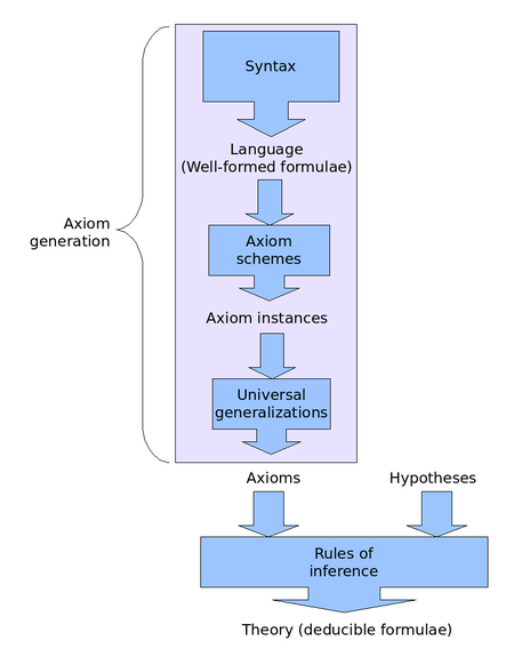
\includegraphics[scale=0.4]{hilbert}
  \caption{A Basic Deduction System}
\end{figure}

The Deduction system is well characterized by use of numerous Logical Axioms called an \textbf{Axiom Scheme}. It gives us a iterative and inductive nature of axiom deduction so that it can be extended as many step as one wish. The terms called \textit{Combinators} (like $\rightarrow$) that interweave the results of a set of a given Axiom Scheme and \textit{Quantifiers} (like $\forall$ ) generalize the results of axiom schemes using some quanitfiable data like the initial value of a mathematical function. 

Using Combinators and Quantifiers one may easily reduce the deductions into less number of steps hence forming metatheorems. A metatheorem inmathematics is the one that can be achieved using some other very basic mathematical theorems. Thus the this gives us idea of correctness of untyped $\lambda$ -calculus. We can thus extend this to other objects also. Below I have tried to explain formation of a Hilbert-style deduction system for Abstract Binding Tree.\\     


Professor \textbf{Robert Harper} in his book \textit{Practical Foundations of Programming Languages} defines the term \textit{Judgement} 'J' defined on a set of rules 'R' defined for a type that satisfies a property 'P' (hence forming an Abstract Binding Tree ABT) and it follows an inductive definition 

\[ \dfrac{J_1 J_2 J_3\cdots J_k}{J}\]

where each J$_i$ is some sort of pre-defined abstract judgements or base cases. The set R is a collection of all such J$_i$s. R is also referred to as an \textit{Axiom} if k=0 i.e it is just first judgement to be made. for example :

\[\dfrac{}{zero\quad nat} \quad \quad and \quad \dfrac{a\quad nat}{succ(a)\quad nat}  \]

He explains \textit{Derivabilty} Judjement J$_1$...J$_k$$\vdash$$_R$ K for a given set of rules 'R', with J$_i$ and K as basic judgements to show that we may derive K from the expansion of R$\cup$\{J$_1$...J$_k$\} of the rules with axioms 

\[ \dfrac{}{J_1} \quad \dfrac{}{J_2} \quad  \dfrac{}{J_3} \quad \cdots \quad \dfrac{}{J_k}   \]

$\Gamma\vdash$$_R$K means that a Judgement K is derivable from rules R$\cup\Gamma$.

He defines \textit{Admissibility} Judgement written as $\Gamma\models_R$J, that if there exists any judgement like $\vdash$$_R$$\Gamma$ then it implies $\vdash$$_R$ J . It means that if all the assumptions (base cases) are derivable from R then J is derivable from R.

The mathemetical formalization of static part and dynamic part of a typed programming language is expressed in the form of the judgements.

The static feature of a language imposes constraints on the formation of the phases that are sensitive to the context in which thay occur. It follows an induction definiton like this

\[\chi | \Gamma\vdash e:\tau\]

where $\chi$ is a finite set of variables and $\Gamma$ is a typing context consisting of hypothesis of the form x:$\tau$, one for each $x\in\chi$. The Dynamics feature basically means the transition of states expressed in form of \textit{Transition} Judgement having a transition $s\longmapsto^n s'$ (for n$^{th}$ order transition) as

\[\dfrac{}{s\longmapsto^n s'} \quad \quad and \quad \dfrac{{s\longmapsto s'} \quad {s'\longmapsto^{*} s"}}{s\longmapsto^{*} s"}  \]

It is important to note that all this operations are performed on pressumed abstract mathematical objects, Abstract Binding Trees (ABTs) which are also the most important fundamental part of any type system. This theoretical equivalence thus allows us to construct the static and dynamic rules and some derived Judgements or abstract functions (with type correctness) for a programming language.

\section{Curry-Howard Correspondence}
In programming language theory the \textbf{Curry–Howard correspondence} (also known as the Curry–Howard isomorphism ) says that mathematical proofs and computer programs are equivalent. This equivalence depends on \textit{Axiom Schemes} with a Type as a combinator. It also follows the \textit{Combinatory Logic System} that allows removing a mentioned variable using some 'ways'. These ways also called functions and they use some combinators to define a result from given arguments. Then it assumes the correctness of Typed-$\lambda$ Calculus. 

Let's assume a function $F$ that has a Type defined by set of rules $R$ and some set of initial conditions J$_i$ (i=1$\cdots n$) then we can write :

\[F \quad \equiv \quad J_{1 \cdots n}\vdash_R \lambda \quad (\lambda \mbox{ is the result of function that also has a Type defined by R.}) \]

A computer program is a set of such functions and a computer aided proof is a computer program. Thus it can be derived that "\textit{A computer Proof is a program with the thesis being proved is type for that program}" . Thus this forms the basis of proof assistants and Functional Programming. 
